\newcommand{\superscript}[1]{\ensuremath{^{\textrm{#1}}}} %To put in exponant
\newcommand{\subscript}[1]{\ensuremath{_{\textrm{#1}}}} %To put in indic

\documentclass{article}
\usepackage{amsmath}
\usepackage[french]{babel} %Pour écrire en français
\usepackage[T1]{fontenc}
\usepackage[utf8]{inputenc} %For accent in firstname 
\usepackage[style=french]{csquotes}
\usepackage{multirow} %For multirow in tables
\usepackage{multicol} %For a multicolumn part in the document
\usepackage{graphicx}
\usepackage{rotating} %figure in landscape
\usepackage{subfig}
\usepackage{fullpage}
\usepackage{pdfpages}
\usepackage[citestyle=authoryear, backend=biber, natbib=true]{biblatex}
\addbibresource{database.bib}

\usepackage{placeins}

\title{Quelques éléments de thermodynamique humide}
\author{Sébastien Riette}
\date{18 octobre 2021}

\begin{document}

\maketitle

\begin{abstract}
Ce document regroupe quelques notions élémentaires de thermodynamique humide.
Si vous y trouvez des erreurs, merci de me le signaler (sebastien.riette@meteo.fr).
La dernière version du document peut être trouvée dans le répertoire /cnrm/phynh/data1/riette/Public/thermo.
\end{abstract}

\tableofcontents

\section{Hypothèses et notations}
\label{sec:hypotheses_notations}
On suppose les gaz parfaits.

On suppose la relation de Clausius-Clapeyron: $\frac{{\rm d} e_s}{{\rm d} T}=\frac{L e_s}{T^2 R}$

Les différentes variables utilisées sont listées dans le tableau \ref{tab:hypotheses_notations:variables}.

Les différentes espèces considérées sont les suivantes:
\begin{itemize}
 \item l'air sec (variables indexées par d - pour dry -)
 \item la vapeur d'eau (variables indexées par v)
 \item les espèces liquides condensées (variables indexées par l)
 \item les espèces solides condensées (variables indexées par i)
\end{itemize}
On utilise également la lettre x pour désigner une espèce quelconque ainsi que la lettre t pour la somme de toutes les espèces en dehors de l'air sec.

\begin{table}[ht]
 \centering
 \begin{tabular}{|c|c|l|}
 \hline
 Symbole   & Unité               & Description \\
 $Cp_d$    & J/Kg/K              & Chaleur massique de l'air sec \\
 $Cp_v$    & J/Kg/K              & Chaleur massique de la vapeur d'eau \\
 $Cp_l$    & J/Kg/K              & Chaleur massique de l'eau liquide \\
 $Cp_i$    & J/Kg/K              & Chaleur massique de la glace \\
 $Cp$      & J/Kg/K              & Chaleur massique du mélange air sec/vapeur à pression constante \\
 $Cph$     & J/Kg/K              & Chaleur spécifique du mélange air sec/vapeur à pression constante \\
 $e$       & Pa                  & Pression partielle de vapeur d'eau \\
 $e_s$     & Pa                  & Pression partielle de vapeur d'eau saturante \\
           &                     & (soit par rapport à l'eau liquide, soit par rapport à la glace) \\
 $e_{sl}$  & Pa                  & Pression partielle de vapeur d'eau saturante par rapport à l'eau liquide \\
 $e_{si}$  & Pa                  & Pression partielle de vapeur d'eau saturante par rapport à la glace \\
 $Hu$      & 0-1 ou 0-100\%      & Humidité relative \\
 $L_v$     & J/Kg                & Chaleur latente de vaporisation \\
 $L_{v_0}$ & J/Kg                & Chaleur latente de vaporisation à T=T0 \\
 $L_s$     & J/Kg                & Chaleur latente de sublimation \\
 $L_{s_0}$ & J/Kg                & Chaleur latente de sublimation à T=T0 \\
 $m$       & Kg                  & Masse \\
 $P_d$     & Pa                  & Pression partielle de l'air sec \\
 $P$       & Pa                  & Pression totale \\
 $q$       & Kg/Kg               & Contenu spécifique (masse d'une espèce par rapport à la masse totale) \\
 $r$       & Kg/Kg               & Rapport de mélange (masse d'une espèce par rapport à la masse d'air sec) \\
 $R_v$     & J/kg/K              & Constante des gaz parfaits pour la vapeur d'eau \\
 $R_d$     & J/kg/K              & Constante des gaz parfaits pour l'air sec \\
 $R$       & J/kg/K              & ``Constante'' des gaz parfaits du mélange air sec/vapeur \\
 $R^*$     & J/kg/K              & ``Constante'' des gaz parfaits du mélange air sec/vapeur à utiliser avec $\rho_d$ \\
 $T$       & K                   & Température \\
 $T0$      & K                   & Constante valant 273.16K (point triple) \\
 $TT$      & K                   & Constante valant 273.15K \\
 $V$       & m\superscript{3}    & Volume \\
 $\rho_d$  & kg/m\superscript{3} & Masse volumique de l'air sec \\
 $\rho_v$  & kg/m\superscript{3} & Masse volumique de la vapeur d'eau \\
 $\rho$    & kg/m\superscript{3} & Densité de l'air humide \\
 $\theta$  & K                   & Notation utilisée pour les différentes températures potentielles \\
 \hline
 \end{tabular} 
 \caption{Liste des variables. À noter que beaucoup d'entre elles peuvent être indexées par l'espèce concernée.}
 \label{tab:hypotheses_notations:variables}
\end{table}
\FloatBarrier

\section{Équilibre entre les phases}
\label{equilibre_phases}
L'intégration de la relation de Clausius-Clapeyron, donne (voir également figure \ref{fig:equilibre_phases:diag_eau}):
\begin{itemize}
 \item {\color{red}$e_{sl}(T) = exp(\alpha_l-\beta_l/T-\gamma_l ln(T))$} avec $\gamma_l=(Cp_l-Cp_v)/R_v$, $\beta_l=L_{v_0}/R_v+T0 \gamma_l$ et $\alpha_l$ tel que $e_{sl}(T0)=611.14$
 \item {\color{red}$e_{si}(T) = exp(\alpha_i-\beta_i/T-\gamma_i ln(T))$} avec $\gamma_i=(Cp_i-Cp_v)/R_v$, $\beta_i=L_{s_0}/R_v+T0 \gamma_i$ et $\alpha_i$ tel que $e_{si}(T0)=611.14$
\end{itemize}
L'humidité relative est alors définie par $Hu_l=100 e /e_{sl}$ ou $Hu_i=100 e /e_{si}$.

\begin{figure}[ht]
  \centering
  \subfloat[Diagramme de phase de l'eau]{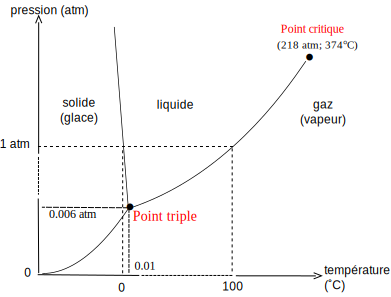
\includegraphics[width=0.45\textwidth]{Diag_eau}}
  \subfloat[Comparaison $e_{sl}$ et $e_{si}$]{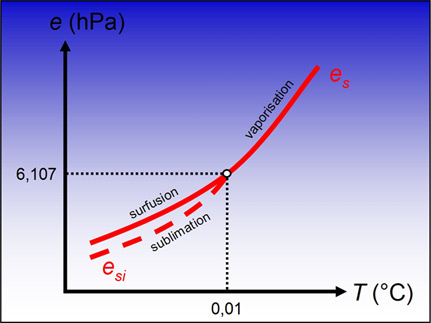
\includegraphics[width=0.45\textwidth]{uved-image-courbes-es2t}}
  \caption{À gauche, diagramme de phase de l'eau où les courbes sont déduites de la relation de Clapeyron (Par Maghémite — Travail personnel, CC BY-SA 3.0, https://commons.wikimedia.org/w/index.php?curid=4047742); à droite, comparaison $e_{sl}$ et $e_{si}$ (http://sup.ups-tlse.fr/uved/Ozone/BasesScientifiques/projet/site/html/ThermodynamiqueAtmosphere\_3.html).}
  \label{fig:equilibre_phases:diag_eau}
\end{figure}

\begin{figure}[ht]
  \centering
  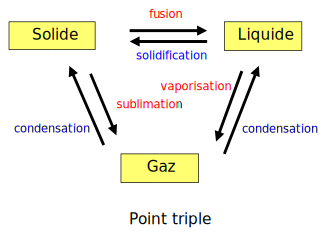
\includegraphics[width=0.7\textwidth]{Point-triple_clapeyron}
  \caption{Noms des changements de phase (Par Maghémite Original uploader was Maghémite at fr.wikipedia — Travail personnel Transferred from fr.wikipedia; Transfer was stated to be made by User:Maghémite., CC BY-SA 2.5, https://commons.wikimedia.org/w/index.php?curid=3984989). En rouge, les noms de processus qui refroidissent l'environnement en absorbant de la chaleur; en bleu ceux réchauffant l'environnement par libération de chaleur.}
  \label{fig:equilibre_phases:vocabulaire}
\end{figure}
\FloatBarrier

\section{Pression, contenus}
\label{pression_contenus}
On a $\rho_x=m_x/V$.

Les contenus utilisés:
\begin{itemize}
 \item $r_x=m_x/m_d=\frac{m_x}{V}\frac{V}{m_d}=\rho_x/\rho_d$
 \item $q_x=m_x/(m_d+m_t)=\frac{m_x}{V}\frac{V}{m_d+m_t}=\rho_x/\rho$ avec $m_t=m_v+m_l+m_i$
\end{itemize}
Il faut noter que l'apport extérieur d'une espèce humide ne change que le rapport de mélange de cette espèce mais modifie, par contre, tous les contenus spécifiques.

Les conversions entre rapports de mélange et contenus spécifiques:
\begin{itemize}
 \item $q_x=\frac{\rho_x}{\rho_d+\rho_t}=\frac{r_x \rho_d}{\rho_d + r_t \rho_d}$ donc {\color{red} $q_x=r_x/(1+r_t)$}
 \item $r_x=\frac{\rho_x}{\rho-\rho_t}=\frac{q_x \rho}{\rho-q_t \rho}$ donc {\color{red} $r_x=q_x/(1-q_t)$}
\end{itemize}
On a également $(1-q_t)(1+r_t)=1$.

L'équation des gaz parfaits s'écrit:
\begin{itemize}
 \item $e=\rho_v R_v T$
 \item $P_d=\rho_a R_d T$
 \item $P=\rho R T$ avec $P_d+e=P$ (les autres hydrométéores ne participent pas à la pression car ils sont non gazeux~; par contre on veut les comptabiliser dans le $\rho$, c'est pourquoi ils doivent apparaître dans le $R$)
 \item {\color{red}$P=\rho_d R^* T$} avec également $P_d+e=P$ (ceci n'est nullement une approximation car on utilise alors $R^*$ et non $R$)
\end{itemize}
On en déduit:
\begin{itemize}
 \item $R=(\rho_d R_d + \rho_v R_v)/\rho=(1-q_v-q_l-q_i)R_d+q_v R_v$ et donc {\color{red}$R=R_d+q_v(R_v-R_d)-q_l R_d -q_i R_d$}
 \item $R=(R_d +r_v R_v)/(1+r_v+r_l+r_i)$
 \item {\color{red}$R^*=R_d + r_v R_v$} (seule la vapeur intervient)
\end{itemize}
Quand les variables sont connues sous forme de contenus spécifiques, on utilise la version avec le vrai $\rho$ et le vrai $R$.
Par contre, quand les variables sont connues sous forme de rapports de mélange, il est plus simple d'utiliser le $\rho_d$ associé à $R^*$.

Les contenus peuvent être exprimés en fonction de $e$ (ce qui permet les conversions avec l'humidité relative):
\begin{itemize}
 \item $r_v=\frac{R_d}{R_v}\frac{e}{P-e}$, si on veut cacluler un rapport de mélange à saturation, il faut distinguer la saturation au dessus de l'eau liquide et au dessus de la glace
 \item $q_v=(1-q_l-q_i)/(1+\frac{R_v}{R_d}(P/e-1))$
\end{itemize}
On a donc aussi:
\begin{itemize}
 \item $e=P r_v / (R_d/R_v +r_v)$
 \item $e=P q_v (R_v/R_d) / (1-q_l-q_i+q_v(R_v/R_d-1))$
\end{itemize}

\section{Chaleurs massique et latente, mélange et changements de phase}
\label{Cp}
\subsection{Chaleur massique}
Lors d'un changement de température, on a $(m_d+m_t)Cp {\rm d}T=(m_d Cp_d + m_v Cp_v + m_l Cp_l + m_i Cp_i){\rm d}T$, donc {\color{red}$Cp=Cp_d(1-q_t)+Cp_v q_v + Cp_l q_l + Cp_i q_i$}.

On écrit également {\color{red}$Cph=(1+r_t)C_p=\frac{Cp}{1-q_t}=Cp_d+Cp_v r_v + Cp_l r_l + Cp_i r_i$}.

\subsection{Chaleur latente}
En passant par le point triple, on a {\color{red}$L_v=L_{v_0}+(Cp_v-Cp_l)(T-T0)$} et {\color{red}$L_s=L_{s_0}+(Cp_v-Cp_i)(T-T0)$}.
On peut aussi écrire ces relations en regroupant les termes constants: $L_v=LV0+(Cp_v-Cp_l)T$ et $L_s=LS0+(Cp_v-Cp_i)T$ avec $LV0=L_{v_0}-(Cp_v-Cp_l)T0$ et $LS0=L_{s_0}-(Cp_v-Cp_i)T0$ à ne pas confondre avec $L_{v_0}$ et $L_{s_0}$.

\subsection{Changements de phases}
Le changement de température dû à un changement de phase (ici entre l'eau liquide et la vapeur), s'écrit~: $(m_a+m_t)Cp{\ \rm d}T=L_v {\ \rm d}m_{v\rightarrow l}$, d'où:
\begin{itemize}
 \item {\color{red}$Cp{\ \rm d}T=L_v{\ \rm d}q_{v\rightarrow l}$}
 \item {\color{red}$Cph{\ \rm d}T=L_v{\ \rm d}r_{v\rightarrow l}$}
\end{itemize}
La première forme est à préférer lorsque les variables sont connues sous forme de contenus spécifiques, la seconde lorsqu'elles sont connues sous forme de rapports de mélange.

Cette relation peut être utilisée pour calculer la température après un changement de phase de plusieurs façons~:
\begin{itemize}
  \item en différences finies avec une résolution explicite~; de cette façon, le $Cp$ et le $L_v$ utilisés sont ceux en début de transformation et cela semble conduire à une sur-estimation de la température lors d'une condensation ou d'une évaporation.
  \item en différences finies avec une résolution implicite
  \item en intégrant la relation de manière analytique au préalable. On obtient alors la relation $\frac{L_v^+}{L_v^-}=\frac{Cp^-}{Cp^+}$ (et en multipliant les $Cp$ par $(1+r_t)$ on a également $\frac{L_v^+}{L_v^-}=\frac{Cph^-}{Cph^+}$) où les exposants $^+$ (resp. $^-$) indiquent les valeurs en fin (resp. en début) de transformation.
\end{itemize}

La dernière possibilité est équivalente à conserver la variable $\chi=CpT-LV0 q_l-LS0 q_i$ où $q_l$ (respectivement $q_i$) contient toutes les espéces liquides (resp. solides). Pour calculer la température lors d'un changement de phase, il faut donc calculer cette variable avant la transformation, calculer les termes $Cp$, $q_l$ et $q_i$ en fin de transformation et en déduire la température. De cette manière la transformation est parfaitement réversible. On peut noter que la variable $(1+r_t)\chi=CphT-LV0 r_l-LS0 r_i$ est également conservée.

\subsection{Mélange}
En utilisant les formules de Pascal Marquet (non reprises ici), on peut vérifier que la conservation de l'enthalpie implique la conservation, par mélange, de la variable $m\chi$.

\section{Températures}
\label{temperatures}

\subsection{Température potentielle}
\label{theta}
La température potentielle d'une particule est la température qu'aurait cette particule si elle subissait une transformation adiabatique ($\delta Q=0$) et sans changement de phase ($R$ et $Cp$ constants) pour l'amener à $P_0$=1000hPa.
La première loi de la thermodynamique semble s'écrire (internet) ${\rm d}h={\rm d}(CpT)+g{\rm d}z=0$. Avec l'utilisation de l'équilibre hydrostatique et de la relation des gaz parfaits, on obtient ${\rm d}P/P=\frac{Cp}{R}{\ \rm d}T/T$.

On a alors $\theta=T(\frac{P_0}{P})^{R_d/Cpd}$ en assimilant l'air à de l'air sec.
On peut poser $Exn=(\frac{P}{P_0})^{R_d/Cpd}$ pour avoir $T=\theta Exn$.

En adiabatique (${\rm d}\theta/{\rm d}z=0$), on a ${\rm d}T/{\rm d}z=-g/Cp\approx-9.75K/km$.

Il semble donc qu'on devrait utiliser les ``vrais'' $Cp$ et $R$. En prenant les valeurs $Cp_d$ et $R_d$, 2 parcelles ayant la même température mais des contenus en vapeur différents auront la même température potentielle alors que cela ne correspond pas à la réalité.

Autre remarque: même si on utilisait les `vrais'' $Cp$ et $R$, la $\theta$ ne devrait pas être utilisée pour calculer la température d'un mélange car elle n'est pas ``corrigée'' du contenu en vapeur. À $P=P_0$, mélanger les $\theta$ revient à mélanger les températures (sans tenir compte des $Cp$ de chacun des constituants du mélange).

\subsection{Température du point de rosée}
\label{Td}
On a $e=e_s(T_d)$.

\subsection{Température (potentielle) pseudo-adiabatique du thermomètre mouillé}
\label{theta_prime_w}

\subsection{Température (potentielle) virtuelle}
\label{theta_v}
La température virtuelle ($T_v$) est la température que doit avoir de l'air sec pour être de même densité que l'air humide considéré. En partant de $P=\rho R T$, on calcule la densité $\rho = \frac{P}{R T} = \frac{P}{R_d T_v}$. On cherche donc $T_v$ telle que $R T = R_d T_v$.

On trouve (avec $R_v / R_d \approx 1.608$)~:
\begin{itemize}
  \item {\color{red}$T_v = (1 + q_v (\frac{R_v}{R_d} - 1) -q_l -q_i) T$}
  \item {\color{red}$T_v = \frac{1 + r_v \frac{R_v}{R_d}}{1 + r_t} T$}
\end{itemize}

La température virtuelle augmente lorsque $r_v$ augmente, l'air humide est moins dense que l'air sec (il se comporte donc comme de l'air sec plus chaud).

On peut alors définir la température potentielle virtuelle.

Note~: certains auteurs réservent le nom de température virtuelle à la température calculée sans tenir compte des condensats~; la température présentée ici est alors appelée "density temperature".

\subsection{Température (potentielle) de l'eau liquide}
\label{theta_l}

\subsection{Température potentielle équivalente}
\label{theta_e}

\end{document}
